\section{Analyse des résultats}
La figure \ref{fig:ResultatsChampsSigma} donnent une illustration des champs des contraintes pour différentes discrétisations. La table \ref{table:objectif} reprend différentes valeurs de l'objectif obtenues pour pour différentes discrétisations. Cette valeur croit bien avec le nombre de triangles, comme prédit par la théorie (voir section Modélisation). 

\begin{table}
\centering
\begin{tabular}{c|cccc}
\textbf{Discrétisation} & $N=4$ & $N=8$ & $N=12$ & $N=16$\\
\textbf{Valeur de l'objectif} & 1.3483 & 1.379409 & 1.3866 & 1.393687 \\
\end{tabular}
\caption{Valeur de l'objectif.}
\label{table:objectif}
\end{table} 

\begin{figure}[h!]
  \centering
  \begin{subfigure}[b]{0.32\textwidth}
  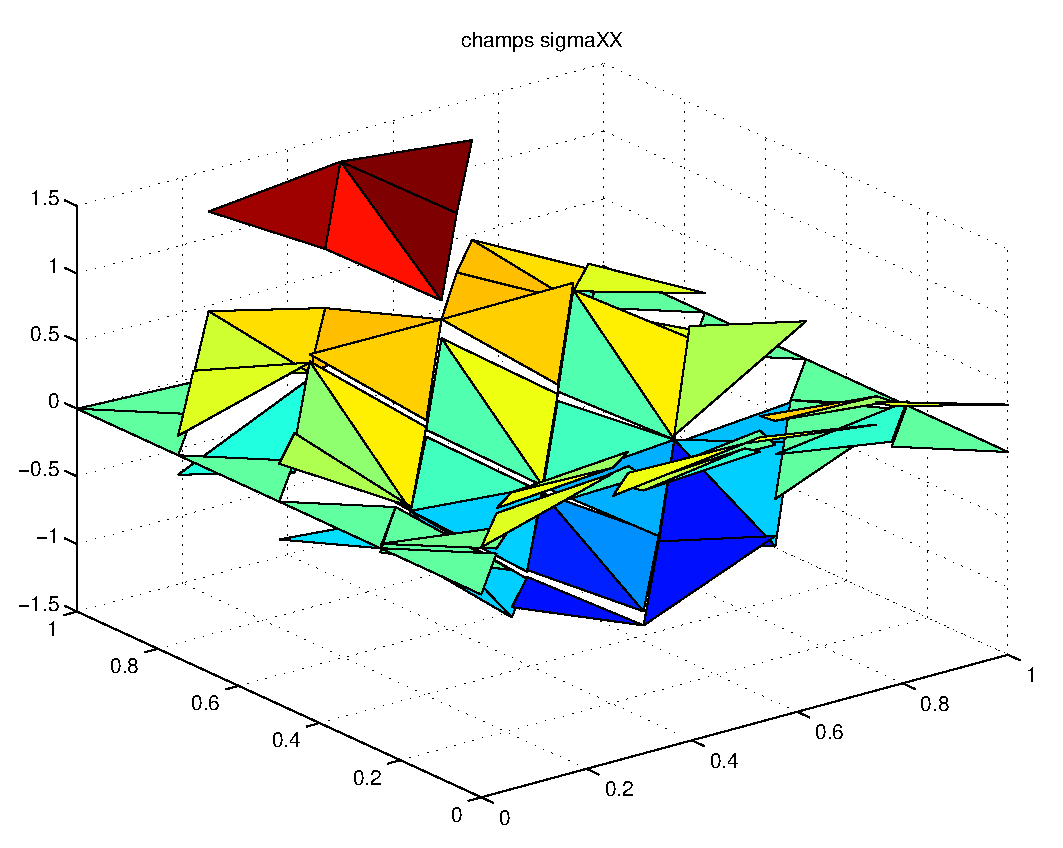
\includegraphics[width=\textwidth]{images/sigmaxxN4.eps}
  \caption{Champs $\sigma_{xx}$ pour $N=4$}
  \end{subfigure}%
  ~
  \begin{subfigure}[b]{0.32\textwidth}
  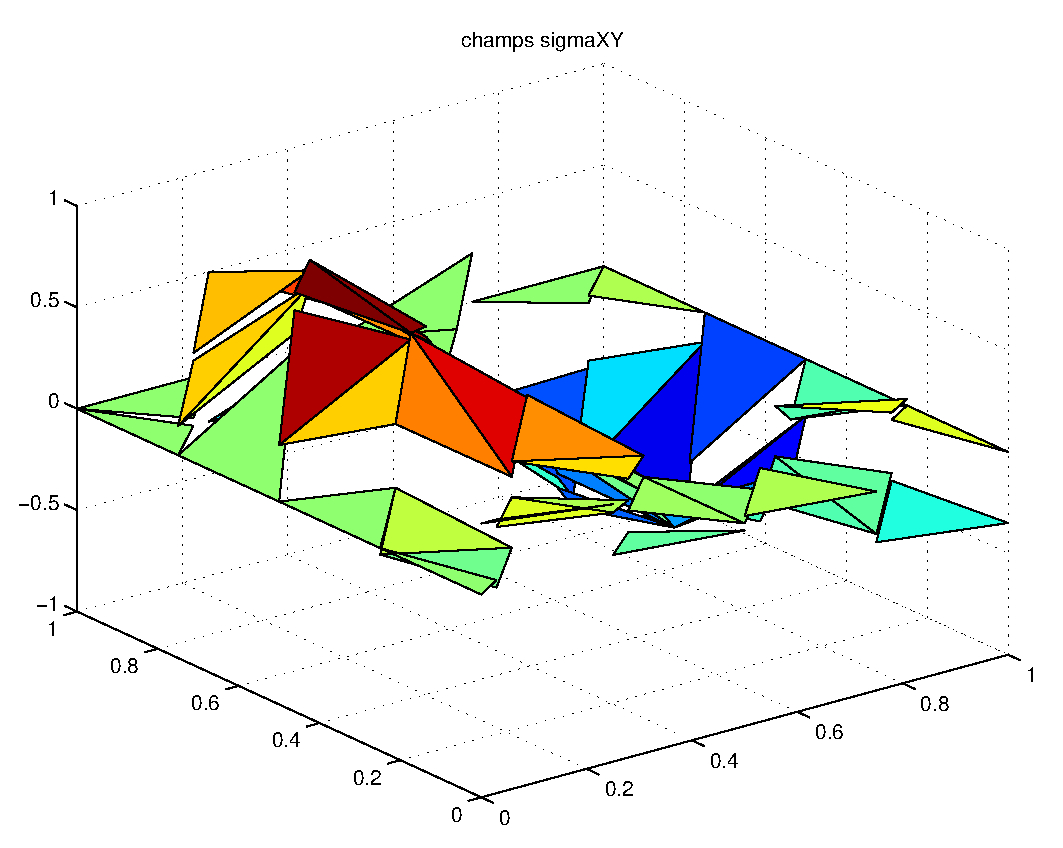
\includegraphics[width=\textwidth]{images/sigmaxyN4.eps}
  \caption{Champs $\sigma_{xy}$ pour $N=4$}
  \end{subfigure}
  ~
  \begin{subfigure}[b]{0.32\textwidth}
  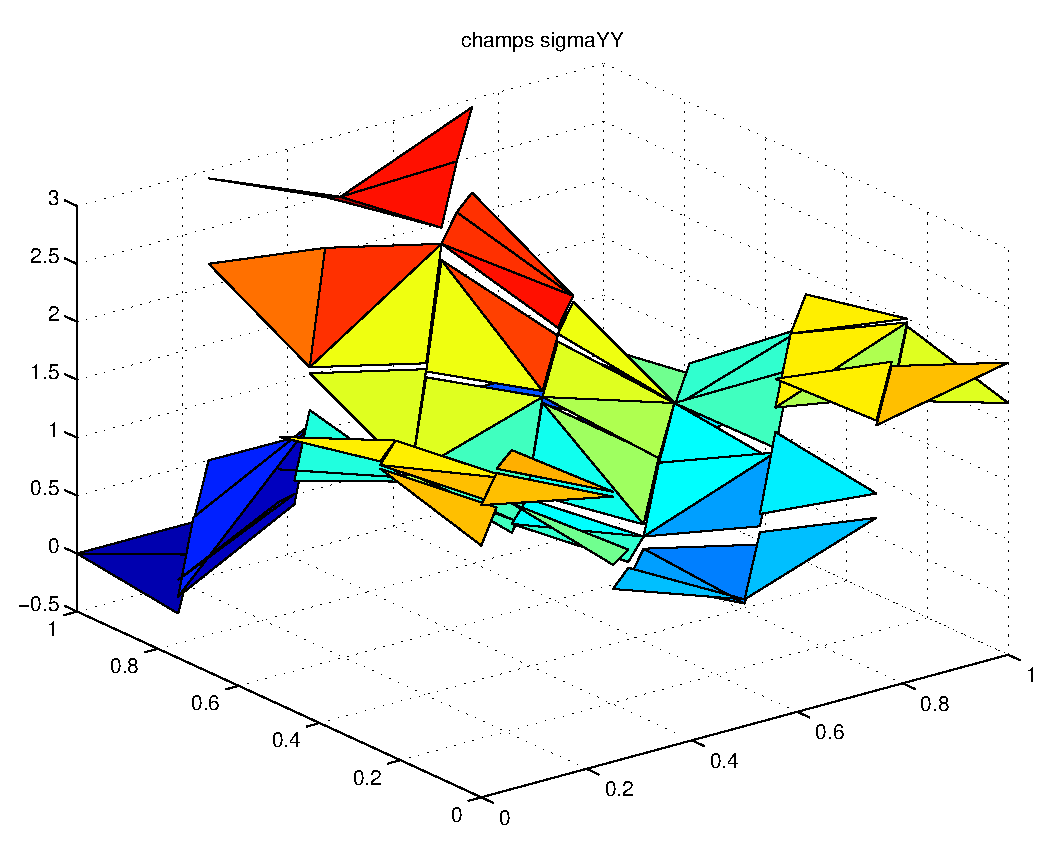
\includegraphics[width=\textwidth]{images/sigmayyN4.eps}
  \caption{Champs $\sigma_{yy}$ pour $N=4$}
  \end{subfigure}
  \begin{subfigure}[b]{0.32\textwidth}
  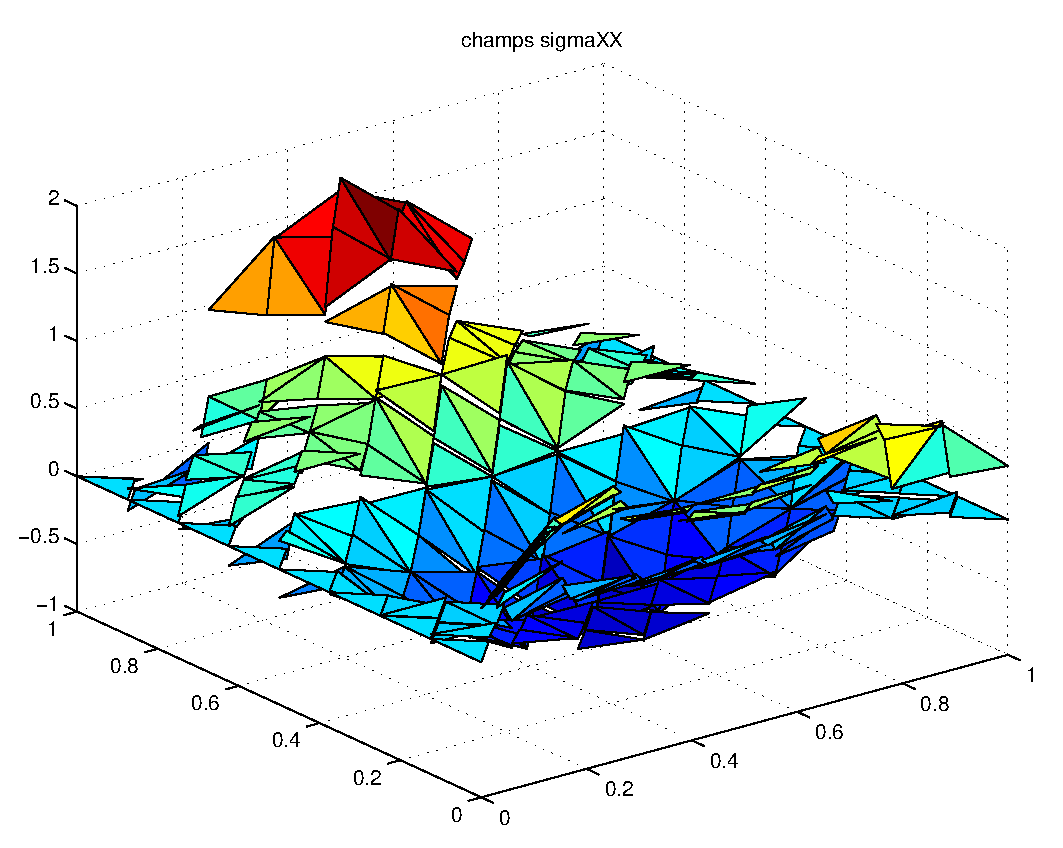
\includegraphics[width=\textwidth]{images/sigmaxxN8.eps}
  \caption{Champs $\sigma_{xx}$ pour $N=8$}
  \end{subfigure}
  ~
  \begin{subfigure}[b]{0.32\textwidth}
  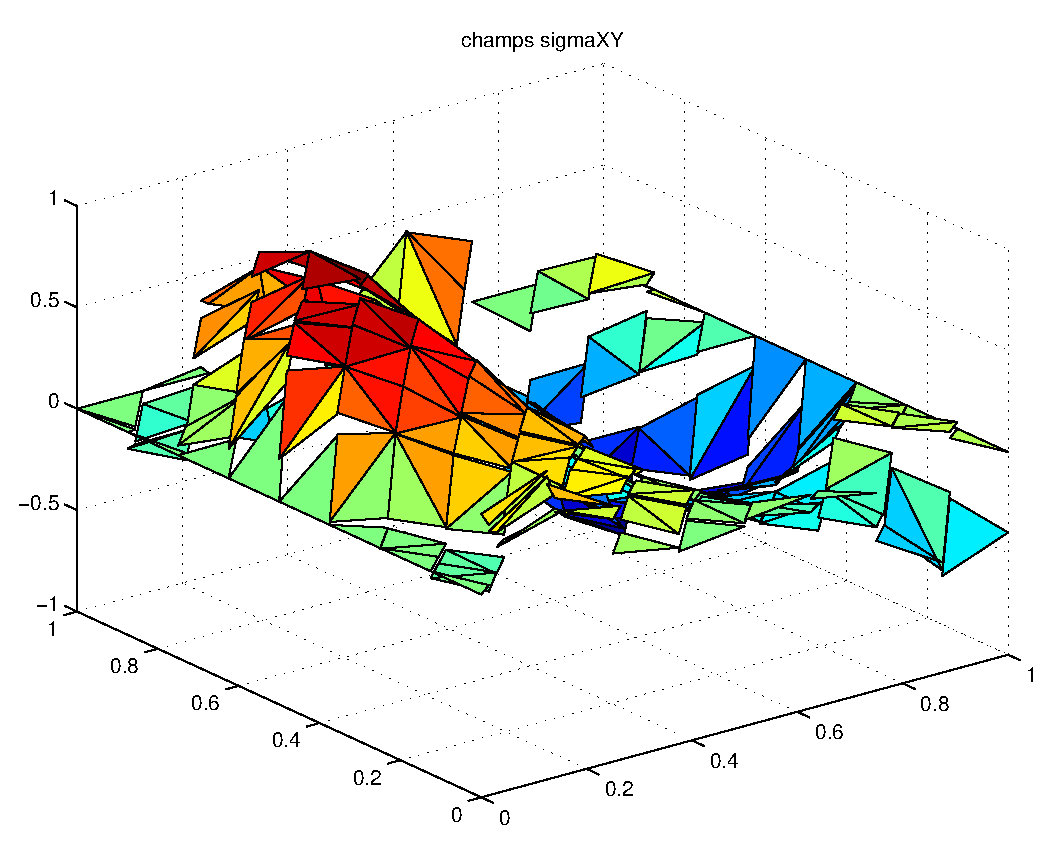
\includegraphics[width=\textwidth]{images/sigmaxyN8.eps}
  \caption{Champs $\sigma_{xy}$ pour $N=8$}
  \end{subfigure}
  ~
  \begin{subfigure}[b]{0.32\textwidth}
  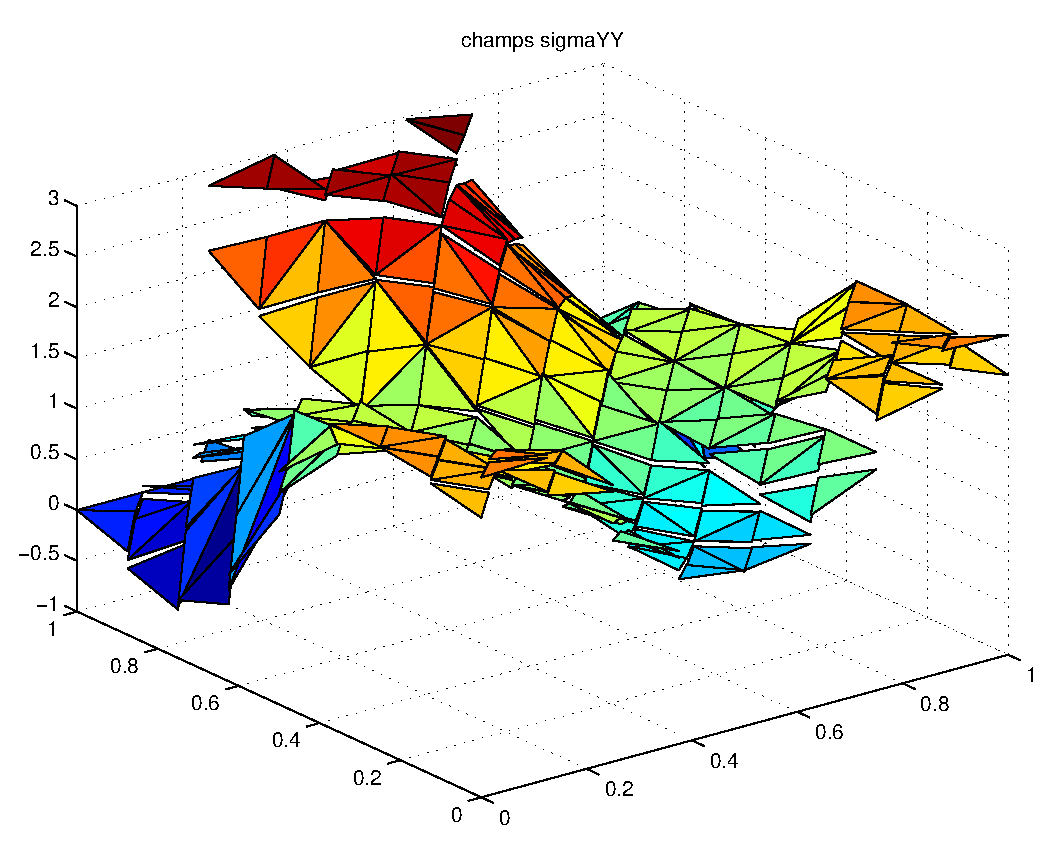
\includegraphics[width=\textwidth]{images/sigmayyN8.eps}
  \caption{Champs $\sigma_{yy}$ pour $N=8$}
  \end{subfigure}
  \begin{subfigure}[b]{0.32\textwidth}
  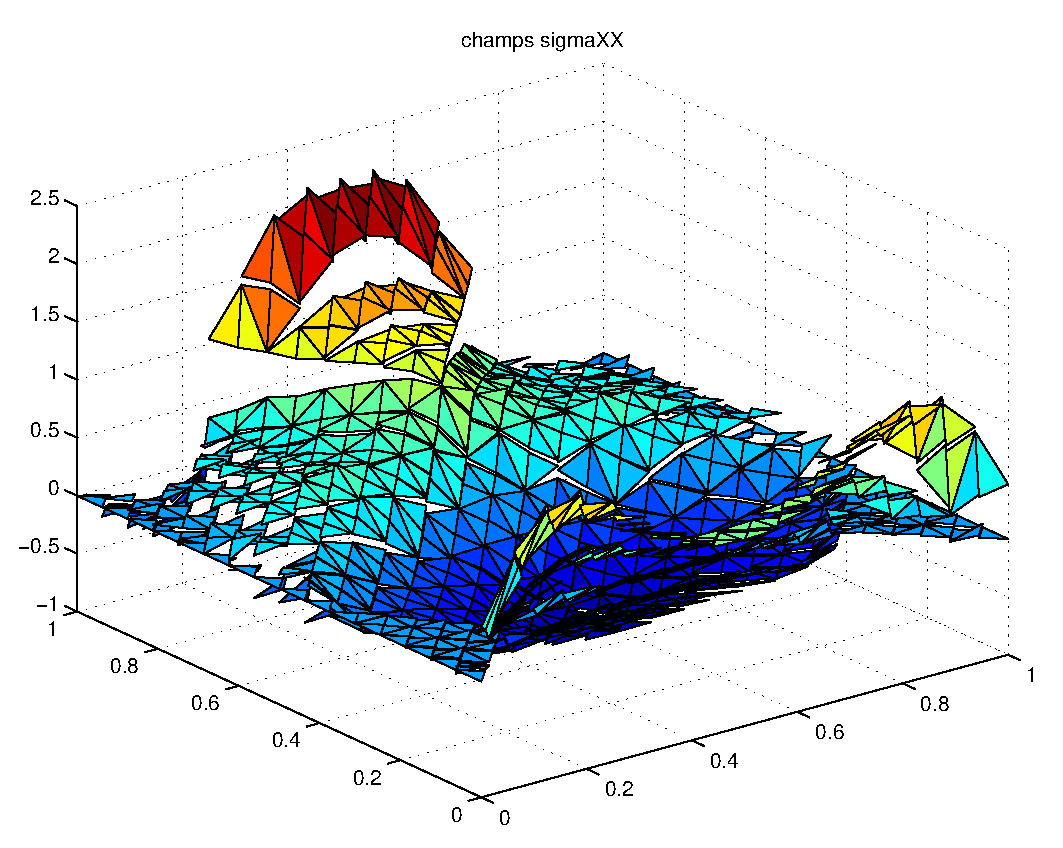
\includegraphics[width=\textwidth]{images/sigmaxxN32.eps}
  \caption{Champs $\sigma_{xx}$ pour $N=16$}
  \end{subfigure}
  ~
  \begin{subfigure}[b]{0.32\textwidth}
  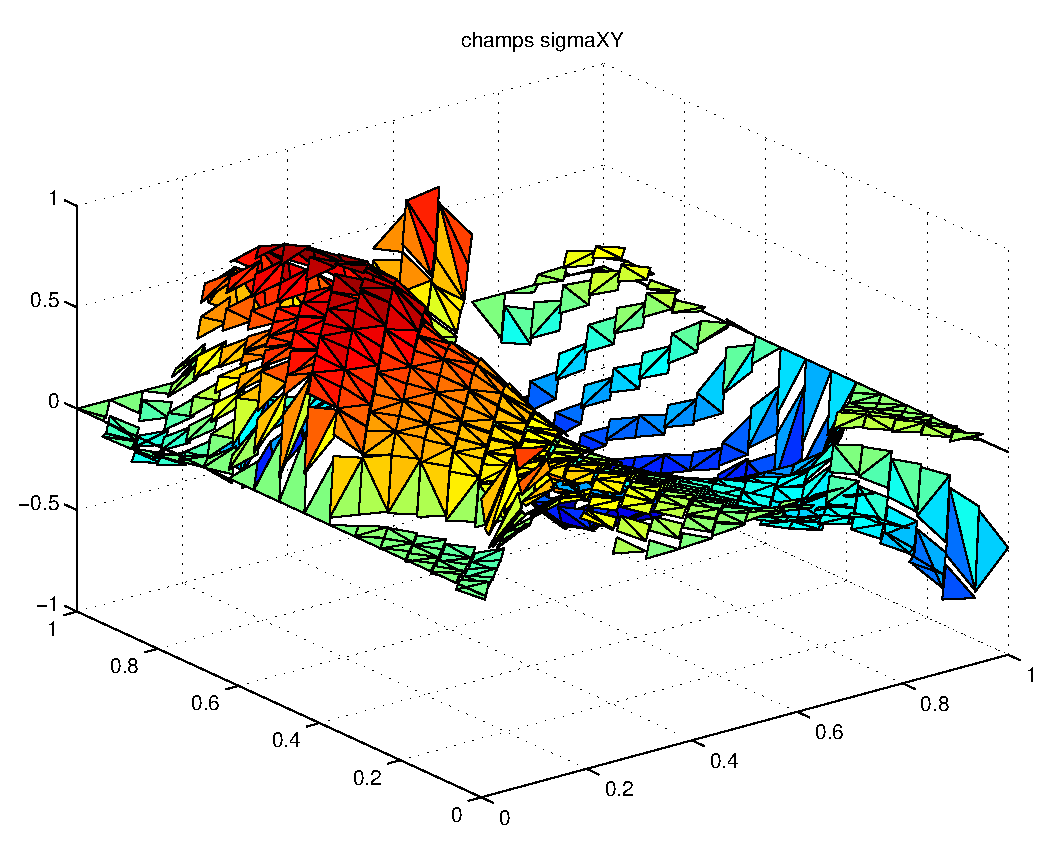
\includegraphics[width=\textwidth]{images/sigmaxyN32.eps}
  \caption{Champs $\sigma_{xy}$ pour $N=16$}
  \end{subfigure}
  ~
  \begin{subfigure}[b]{0.32\textwidth}
  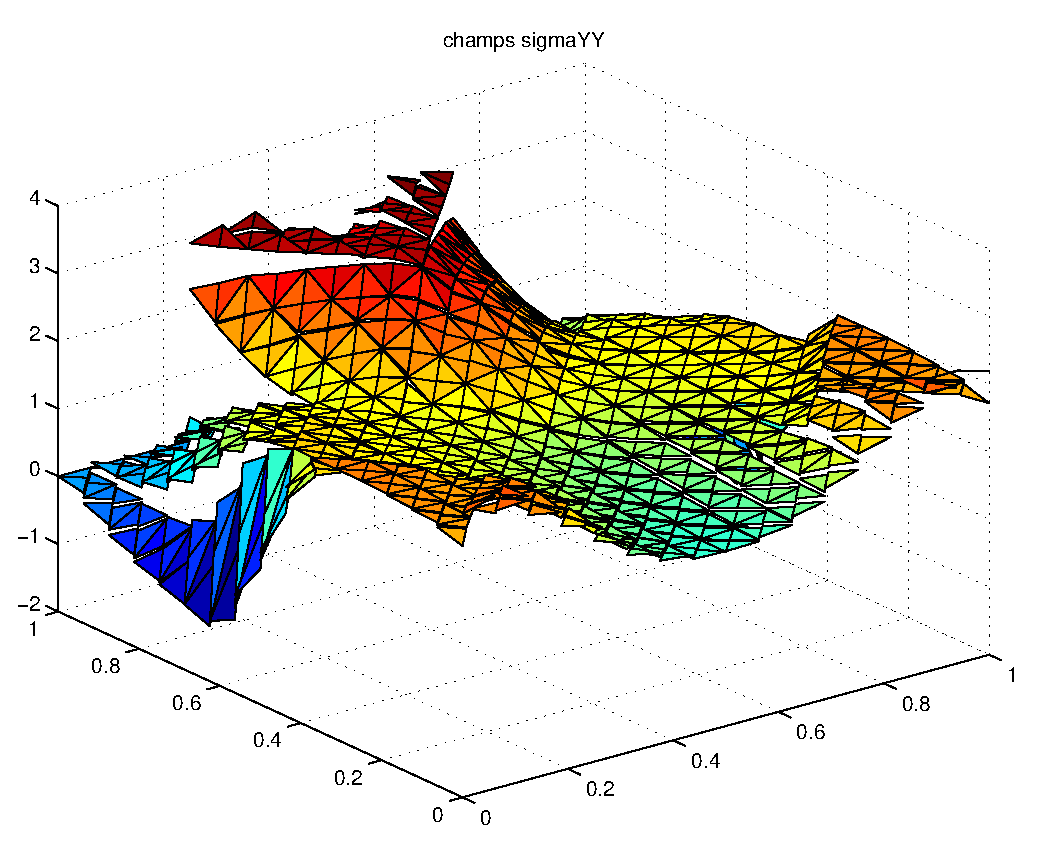
\includegraphics[width=\textwidth]{images/sigmayyN32.eps}
  \caption{Champs $\sigma_{yy}$ pour $N=16$}
  \end{subfigure}
  \caption{}
  \label{fig:ResultatsChampsSigma}
\end{figure}